\documentclass[output=paper]{langsci/langscibook} 
\author{%
	Robert D.\ Borsley\affiliation{University of Essex}%
	\lastand Stefan Müller\affiliation{Humboldt-Universität zu Berlin}%
}
\title{HPSG and Minimalism}

% \chapterDOI{} %will be filled in at production

\maketitle

\begin{document}

\label{chap-minimalism}

\section{Introduction}
\label{sec:min-intro}

The Minimalist\is{Minimalism|(} framework, which was first outlined by Chomsky in the early 1990s
\citep{Chomsky93b-u,Chomsky95a-u}, still seems to be the dominant approach to syntax. It is
important, therefore, to consider how HPSG compares with this framework. The issues are clouded by
the rhetoric that surrounds the framework. At one time ``virtual conceptual necessity'' was said to be
its guiding principle. A little later, it was said to be concerned with the ``perfection of
language'', with ``how closely human language approaches an optimal solution to design conditions
that the system must meet to be usable at all'' \citet[58]{Chomsky2002a-u}. Much of this rhetoric
seems designed to suggest that Minimalism is quite different from other approaches and should not be
assessed in the same way. In the words of Postal \citet[19]{Postal2003a}, it looks like ``an attempt
to provide certain views with a sort of privileged status, with the goal of placing them at least
rhetorically beyond the demands of serious argument or evidence''. However, the two frameworks have
enough in common to allow meaningful comparisons.


Both frameworks seek to provide an account of what is and is not possible both in specific languages and in language in general. Moreover, both are concerned not just with local relations such as that between a head and its complement or complements but also with non-local relations such as those in the following:
\ea\label{ex:min-student-knows}
The student knows the answer.
\z
\ea\label{ex:min-raining}
It seems to be raining,
\z
\ea\label{ex:min-which-student}
Which student do you think knows the answer? 
\z
In (\ref{ex:min-student-knows}), \textit{the student} is subject of \textit{thinks} and is
responsible for the fact that \textit{thinks} is a third person singular form, but they are not
sisters if \textit{knows} and \textit{the answer} form a VP. In (\ref{ex:min-raining}) the subject
is \emph{it} because the complement of \textit{be} is \textit{raining}, but \emph{it} and \emph{raining} are
obviously not sisters. Finally, in (\ref{ex:min-which-student}), \textit{which student} is
understood as the subject of \textit{thinks} and is responsible for the fact that it is third person
singular, but again the two elements are structurally quite far apart. Both frameworks provide
analyses for these and other central syntactic phenomena, and it is quite reasonable to compare them
and ask which is the more satisfactory.% 
	\footnote{As noted below, comparison is complicated somewhat by the fact that Minimalists typically provides only sketches of analyses in which various details are left quite vague.}%

Although HPSG and Minimalism have enough in common to permit comparisons, there are obviously many differences. Some are more important than others, and some relate to the basic approach and outlook, while others concern the nature of grammatical systems and syntactic structures. In this chapter we will explore the full range of differences.

The chapter is organized as follows. In Section~\ref{sec:min-difference}, we look at differences of
approach between the two frameworks. Then in Section~\ref{sec:min-views-grammar}, we consider the
quite different views of grammar that the two frameworks espouse, and in
Section~\ref{sec:min-views-structure}, we look at the very different syntactic structures which
result. Finally, in Section~\ref{sec-psycho}, we consider how the two frameworks relate to
psycholinguistic issues, namely processing and language acquisition.

\section{Differences of approach and outlook}
\label{sec:min-difference}

As many of the chapters in this volume emphasize, HPSG is a framework which places considerable
emphasis on detailed formal analyses of the kind that one might expect within generative
grammar. Thus, it is not uncommon to find lengthy appendices setting out formal analyses. See, for
example, Sag's (\citeyear{Sag97a}) paper on \ili{English} relative clauses\is{relative clause} and especially
\citet{GSag2000a-u}, which has a 50 page appendix. One consequence of this, discussed by
\crossrefchaptert{cl}, is that HPSG has had considerable influence in \isi{computational linguistics}.

In Minimalism things are very different. Detailed formal analyses are virtually non-existent. There
appear to be no appendices like those in \citet{Sag97a} and \citet{GSag2000a-u}. In fact the
importance of \isi{formalization} has long been downplayed in Chomskyan work. Thus, in a 1980
conversation, Chomsky remarked that ``I do not see any point in formalizing for the sake of
formalizing'' (see \citealt[73]{HuybregtsRiemsdijk.1982}), and this view
seems fairly standard within Minimalism (see also \citew[\page 146]{Chomsky90a} and the discussion
in \citew[Section~3.6.2]{MuellerGT-Eng1}). \citet[\page 28]{CL95a-u}
attempt to justify the absence of detailed analyses when they suggest that providing a rule 
system from which some set of phenomena can be derived is not ``a real result'' since ``it is often
possible to devise one that will more or less work''. Instead, they say, `the task is now to show how
the phenomena \ldots{} can be deduced from the invariant principles of UG with parameters set in one
of the permissible ways'. In other words, providing detailed analyses is a job for unambitious
drudges, and real linguists pursue a more ambitious agenda. \citet[5]{Postal2004a-u} comments that
what we see here is ``the fantastic and unsupported notion that descriptive success is not really
that hard and so not of much importance''. He points out that if this were true, one would expect
successful descriptions to be abundant within transformational frameworks. However, he suggests that
``the actual descriptions in these frameworks so far are not only not successful but so bad as to
hardly merit being taken seriously''. Postal does much to justify this assessment with detailed
discussions of Chomskyan work on strong crossover phenomena and passives in
Chapters~7 and~8 of his book. 

There has also been a strong tendency within Minimalism to focus on just a subset of the facts in
whatever domain is being investigated. As \citet[535]{CJ2005a} note, ``much of the fine detail of
traditional constructions has ceased to garner attention''. This tendency has sometimes been
buttressed by a distinction between core grammar, which is supposedly a fairly straightforward
reflection of the language faculty, and a periphery of marked constructions, which are of no great
importance and which can reasonably be ignored. However, as \citet{Culicover99a-u} and others have
argued, there is no evidence for a clear cut distinction between core and periphery. It follows that
a satisfactory approach to grammar needs to account both for such core phenomena as
\textit{wh}-interrogatives, relative clauses, and passives but also with more peripheral phenomena
such as the following: 
\eal
\ex It's amazing the people you see here.\label{ex:min-amazing-people}
\ex The more I read, the more I understand.\label{ex:min-read-understand}
\ex Chris lied his way into the meeting.\label{ex:min-chris-meeting}
\zl 
These exemplify the nominal extraposition construction (\citealt{ML96a}), the comparative correlative construction \citet{Borsley2011a-u}, and the \textit{X's Way} construction (\citealt{Sag2012a}). As has been emphasized in other chapters, the HPSG system of types and constraints is able to accommodate broad linguistic generalizations and highly idiosyncratic facts and everything in between.

The general absence in Minimalism of detailed formal analyses is quite important. It means that Minimalists may not be fully aware of the complexity of the structures they are committed to and allows them to sidestep the question whether it is really justified. It also allows them to avoid the question of whether the very simple conception of grammar that they favour is really satisfactory. Finally, it may be that they are unaware of how many phenomena remain unaccounted for. These are all important matters. 

The general absence of detailed formal analyses has also led to Minimalism having little impact on
computational linguistics. There has been some work that has sought to implement Minimalist ideas
\citep{Stabler2001a,FG2012a,Fong2014a}, but Minimalism has not had anything like the productive
relation with computational work that HPSG has enjoyed. Existing Minimalist implementations are rather toy
grammars analyzing very simple sentences and some do not even do this and require pre-segmented
input. See \citet[Section~4.7.2]{MuellerGT-Eng1} for discussion.

There are, then, issues about the quantity of data that is considered in Minimalist work. There are
also issues about its quality. Research in HPSG is typically quite careful about data and often
makes use of corpus and experimental data (see \citealt{AA2017a-u,Mueller99a,Mueller2002b,BC2010a,MBC2012a}
for examples of work with attested examples and for experimental\is{experiment} work). This use of corpus data and
attested examples is based on the insight that \isi{introspection} alone is not sufficient, given that an
enormous amount of time is spent to work out analyses and it would be unfortunate if these analyses
were build on a shaky empirical basis. See \citew{Mueller2007c} and \citew{MM2009a} for the
discussion of introspection vs.\ corpus data.
Research in Minimalism is often rather less
careful.\footnote{
 We hasten to say that we do not claim this to be true for all Minimalist work. There are
 researchers working with corpora or at least with attested examples \citep{Wurmbrand2003a} and
 there is experimental work. Especially in Germany there were several large scale Collaborative
 Research Centers with a strong empirical focus which also fed back into theoretical work, including
 Minimalist work. The fact that we point out here is that there is work, including work
 by prominent Minimalists, that is rather sloppy as far as data is concerned.%
} In a review of a collection of Minimalist papers, \citet[434]{Bender2002a} comments that: ``In
these papers, the data appears to be collected in an off-hand, unsystematic way, with unconfirmed
questionable judgments often used at crucial points in the argumentation''. She goes on to suggest
that the framework encourages ``lack of concern for the data, above and beyond what is unfortunately
already the norm in formal syntax, because the connection between analysis and data is allowed to be
remote.'' Similar things could be said about a variety of Minimalist work. Consider, for example,
\citet{AounLi.2003}, who argue for quite different analyses of \textit{that}-relatives and
\textit{wh}-relatives on the basis of the following (supposed) contrasts, which appear to represent
nothing more than their own judgements (p.\,110--112):
%\inlinetodostefan{dialectal variation}
\eal
\judgewidth{?*}
\ex[]{The headway that Mel made was impressive.}\label{ex:min-headway-that}
\ex[??]{The headway which Mel made was impressive.}\label{ex:min-headway-which}
\zl
\eal
\judgewidth{?*}
\ex[]{
We admired the picture of himself that John painted in art class.
}\label{ex:min-admire-that}
\ex[*]{
We admired the picture of himself which John painted in art class.
}\label{ex:min-admire-which} 
\zl
\eal
\judgewidth{?*}
\ex[]{The picture of himself that John painted in art class is impressive.}\label{ex:min-picture-that}
\ex[*?]{The picture of himself which John painted in art class is impressive.}\label{ex:min-picture-which} 
\zl
None of the native speakers we have consulted find significant contrasts here which could support
different analyses. The example in (\mex{1}a) with a \emph{which} relative clause referring to \emph{headway} can be found in
\citew{CHH82a-u}, \citew[\page 437]{Williams89a-u} and \citew[\page 221]{Falk2010a-u} have examples
with a reflexive coreferential with a noun in a relative clause introduced by \emph{which} as in
William's (\mex{1}b) and corpus examples like (\mex{1}c,d) can be found as well:
%\inlinetodostefan{BB: We need examples where a which relative has an antecedent containing a reflexive and the antecedent is inside the relative. Tom Wasow's examples look good to me.}
\ealnoraggedright
\ex The headway which we made was satisfactory.
\ex the picture of himself which John took

\ex The words had the effect of lending an additional clarity and firmness of outline to the picture
    of himself which Bill had already drawn in his mind--of a soulless creature sunk in hoggish
    slumber.\footnote{
      Wodehouse, P.G. 1917. \emph{Uneasy Money}, London: Methuen \& Co., p.\,186,
      \url{http://www.literaturepage.com/read.php?titleid=uneasymoney&abspage=186},
      2018-09-18.
}
\ex She refused to allow the 
picture of himself, which he had sent her, to be hung, 
and it was reported that she ordered all her portraits 
and busts of him to be put in the lumber attics.\footnote{
 Jerrold, Clare. 1913. \emph{The married life of Queen Victoria}, London: G.\ Bells \& Sons, Ltd.
 \url{https://archive.org/stream/marriedlifeofque00jerruoft/marriedlifeofque00jerruoft_djvu.txt}, 2018-09-19.
}
%% \ex The words had the effect of lending an additional clarity and firmness of outline to the picture
%% of himself which Bill had already drawn in his mind--of a soulless creature sunk in hoggish
%% slumber.\footnote{
%% Wodehouse, P.G. 1917. \emph{Uneasy money}. London: Methuen \& Co. \url{http://www.freeclassicebooks.com/P.G.\%20Wodehouse/Uneasy\%20Money.pdf}, 2018-09-19.
%% }

%% \ex Like Milton, Calvin believed that the scriptural presentation of God should be accepted as the
%%     picture of himself which God wished people to perceive \ldots\footnote{
%%   Neil D. Graves. 2001. \emph{Milton and the Theory of Accommodation}, Studies in Philology,
%%   Vol. 98, No. 2.
%% }
\zl
%Also in Yehuda N. Falk On the Syntactic Analysis of Relative Clauses
%
Given that it is relatively easy to come up with counter examples it is surprising that authors do
not do a quick check before working out rather complex analyses.

Note that we are not just taking one bad example of Minimalist work. It is probably the case that
papers with dubious judgments can be found in any framework if only this is due to the repetitions
of unwarranted claims made by others. The point is that Aoun \& Li are influential (quoted by 455
other publications as of 2018-09-14). Others rely on these judgments or the analyses that were
motivated by them. New conclusions are derived from analyses since theories make predictions. If
this process continues for a while an elaborated theoretical building results that is not
empirically supported. Note furthermore that the criticism raised here is not the sqabble of two
authors working in an alternative framework. This criticism also comes from practitioners of
Mainstream Generative Grammar. For example, Wolfgang Sternefeld and Hubert Haider, both very
prominent figures in the German Generative Grammar school criticized the scientific standards in
Minimalism heavily \citep{%Ross2011a,
SR2012a,Haider2018a}. As \citet[\page 266--268]{SR2012a} point out it is not
just the case that Minimalist publications are based on empirically problematic foundations, it is
even worse: researchers like \citet[Section~1.1]{ES2006a-u} publish statements about research
methodology that can only be understood as an immunization strategy. The authors discuss the two
curves in Figure~\ref{fig-immunization-MP}:
one has a sinus-like shape and hits three out of seven of the data points on a straight line and the
other one is parallel to the line with the data points and hence hits none of the data points. The
second approach gets none of the data right. Nevertheless the authors argue that one should prefer
this theory since it was closer to the truth and more illuminating: ``Clearly, Theory~1 is
`empirically preferable’ by a `winning score’ of 3--0. The point [\ldots] is that Theory~2, despite
getting none of the data correct, [\ldots] is `closer to the truth’ or `more illuminating’ than the
empirically preferable Theory~1. Hence, we believe, Theory~2 is a better working or guiding
hypothesis upon which to base future research.'' \citep[\page 2]{ES2006a-u}
\begin{figure}
\begin{subfigure}{0.48\textwidth}
\scalebox{.78}{%
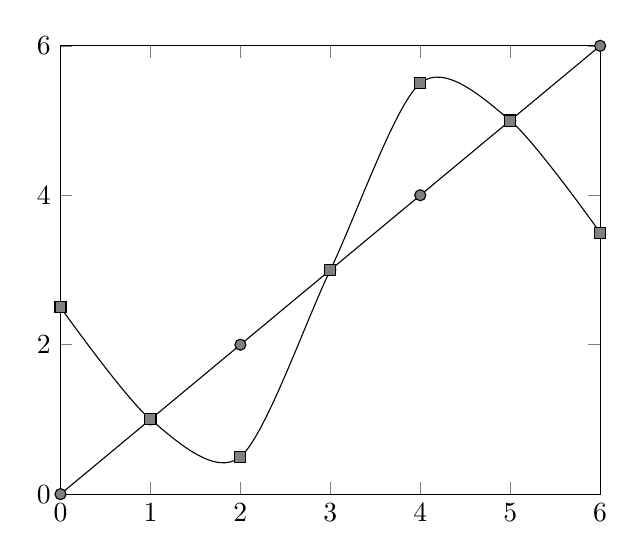
\begin{tikzpicture}
    \begin{axis}[
        xmin=0,xmax=6,
        ymin=0,ymax=6,
        cycle list name=black white
    ]
    \addplot+ [sharp plot] coordinates {(0,0) (1,1) (2,2) (3,3) (4,4) (5,5) (6,6)};
    \addplot+ [smooth]     coordinates {(0,2.5) (1,1) (2,0.5) (3,3) (4,5.5) (5,5) (6,3.5)};
        \end{axis}
\end{tikzpicture}}
\caption{Theory 1}
\end{subfigure}
\hfill
\begin{subfigure}{0.48\textwidth}
\scalebox{.78}{%
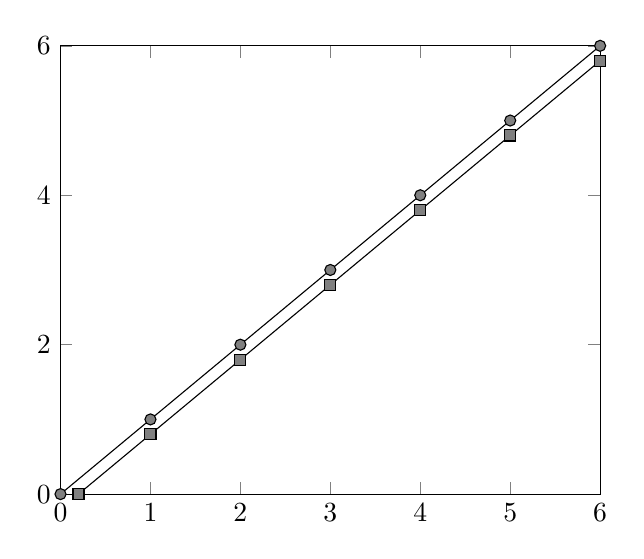
\begin{tikzpicture}
    \begin{axis}[
        xmin=0,xmax=6,
        ymin=0,ymax=6,
        cycle list name=black white
    ]
    \addplot+ [sharp plot] coordinates {(0,0) (1,1) (2,2) (3,3) (4,4) (5,5) (6,6)};
    \addplot+ [sharp plot] coordinates {(0.2,0) (1,.8) (2,1.8) (3,2.8) (4,3.8) (5,4.8) (6,5.8)};
        \end{axis}
\end{tikzpicture}}
\caption{Theory 2}
\end{subfigure}
\caption{\label{fig-immunization-MP}Immunization in Minimalist work: According to \citet[Section~1.1]{ES2006a-u} Theory~2, which gets none of the data points, is
  preferable to Theory~1 with three data points since Theory~2 is ``more illuminating'' and ``closer to
  to the truth''}
\end{figure}


There are also differences in the kind of arguments that the two frameworks find acceptable. It is
common within Minimalism to assume that some phenomenon which cannot be readily observed in some
languages must be part of their grammatical system because it is clearly present in other
languages. Notable examples would be case or agreement. This stems from the longstanding Chomskyan
assumption that language is the realization of a complex innate language faculty. From this
perspective, there is much in any grammatical system that is a reflection of the language faculty
and not in any simple way of the observable phenomena of the language in question. If some
phenomenon plays an important role in many languages it is viewed as a reflection of the language
faculty, and hence it must be a feature of all grammatical systems even those in which it is hard to
see any evidence for it. An example -- taken from a textbook on Minimalism \citep*[\page
  124]{HNG2005a} -- is an analysis of prepositional phrases in
English. Figure~\ref{fig-understnading-Minimalism-PP} shows the analysis.
\begin{figure}
\centering
\begin{forest}
sm edges
[AgrP
  [DP [me$_j$]]
  [Agr$'$
    [Agr [with$_j$]]
    [PP
      [P$'$
        [P [\trace$_i$]]
        [DP [\trace$_j$]]]]]]
\end{forest}
\caption{\label{fig-understnading-Minimalism-PP}Minimalist analysis of a PP according to \citep*[\page 124]{HNG2005a}}
\end{figure}
Due to theory internal assumptions the case requirement of the preposition cannot be checked in the
P-DP combination. According to the version of the theory adopted by the authors, case has to be
checked in specifier positions. Therefore it was assumed that the preposition moves to an Agr head
and the DP moves to the specifier position of this Agr head. The problem is of course that DP and P
are in the wrong order now. However, the authors argue that this is the order that is manifested in
\ili{Hungarian} and that Hungarian is a language which has postpositions and these are agreeing with
their nominal dependent. It is claimed that the movement exists both in Hungarian and in English but
that the movement is covert (that is, invisible) in the latter language.

This line of argument would be reasonable if a complex innate language
faculty was an established fact, but it isn't, and since \citet*{HCF2002a}, it seems to have been
rejected within Minimalism.  It follows that ideas about an innate language faculty should not be
used to guide research on individual languages. Rather, as \citet[25]{MuellerCoreGram} puts it,
``grammars should be motivated on a language-specific basis''. Does this mean that other languages are
irrelevant when one investigating a specific language? Clearly not. As \Citeauthor{MuellerCoreGram}
also puts it, ``In situations where more than one analysis would be compatible with a given dataset
for language X, the evidence from language Y with similar constructs is most welcome and can be used
as evidence in favor of one of the two analyses for language X.'' (\citeyear[43]{MuellerCoreGram}). In
practice, any linguist working on a new language will use apparently similar phenomena in other
languages as a starting point. It is important, however, to recognize that apparently similar
phenomena may turn out on careful investigation to be significantly different.\footnote{%
  Equally, of course, apparently rather different phenomena may turn out on careful investigation to
  be quite similar. For further discussion of HPSG and comparative syntax, see Borsley  (forthcoming).%
} 

\section{Different views of grammar}
\label{sec:min-views-grammar}

We turn now to more substantive differences between HPSG and Minimalism, differences in their conceptions of grammar, especially syntax, and differences in their views of syntactic structure. As we will see, these differences are related. In this section we consider the former, and in the next we will look at the latter.

As is emphasized throughout this volume, HPSG assumes a declarative or constraint-based view of
grammar. It also assumes that the grammar involves a complex systems of types and
constraints. Finally, it assumes that syntactic analyses are complemented by separate semantic and
morphological analyses. In each of these areas, Minimalism is different. It assumes a procedural
view of grammar. It assumes that grammar involves just a few general operations. Finally, it assumes
that semantics and morphology are simple reflections of syntax. We comment on each of these matters
in the following paragraphs. 

Whereas HPSG is a declarative or constraint-based approach, Minimalism seems to be firmly committed
to a procedural approach. \citet[219]{Chomsky95a-u} remarks that: ``We take L [a particular language]
to be a generative procedure that constructs pairs (π, λ) that are interpreted at the
articulatory-perceptual (A-P) and conceptual-intentional (C-I) interfaces, respectively, as
`instructions' to the performance systems.''. Various arguments have been presented within HPSG for
a declarative view, but no argument seems to be offered within Minimalism for a procedural
view. Obviously, speakers and hearers do construct representations and must have procedures that
enable them to do so, but this is a matter of performance, and there is no reason to think that the
knowledge that is used in performance has a procedural character. Rather, the fact that it used in
both \isi{production} and \isi{comprehension} suggests that it should be neutral between the two and hence
declarative. For further discussion of the issues, see e.\,g.\ \citet{PS2001a}, \citet{Postal2003a},
\citeauthor{SW2011a} \citeyearpar{SW2011a,SW2015a}, and \crossrefchaptert{processing}.\inlinetodostefan{Bob: Maybe we should say more here.}
The declarative-procedural contrast is an important one, but the contrast between the complex
systems of types and constraints that are assumed within HPSG and the few general operations that
form a Minimalist grammar is arguably more important.\footnote{%
  A procedural approach doesn't necessarily involve a very simple grammatical system. The Standard
  Theory of transformational grammar \citep{Chomsky65a} is procedural but has many different rules,
  both phrase structure rules and transformations.}
Much work in Minimalism has three main operations Merge, Agree, and Move or Internal Merge. Merge\is{Merge!External}
combines two expressions, either words or phrases, to form a larger expression with the same label
as one of the expressions \citep[244]{Chomsky95a-u}. Its operation can be presented as shown in Figure~\ref{fig:min-merge}.
\begin{figure}
\centering
	\raisebox{1\baselineskip}{X, Y $\Rightarrow$}
	\hspace{1em}
	\begin{forest}
		[X [X] [Y]]
	\end{forest}
\hspace{1em}
\raisebox{1\baselineskip}{or}
\hspace{1em}
	\begin{forest}
		[Y [X] [Y]]
	\end{forest}
	\caption{\label{fig:min-merge}Merge}\is{Merge}
\end{figure}
In the case of English, the first alternative is represented by situations where a lexical head
combines with a complement while the second is represented by situations where a specifier combines
with a phrasal head. 

Agree, as one might suppose, offers an approach to various kinds of agreement phenomena. It involves
a probe, which is a feature or features of some kind on head, and a goal, which the head
c-commands. At least normally, the probe is an uninterpretable feature or features with no value and
the goal has a matching interpretable feature or features with appropriate values. Agree values the
uninterpretable feature or features and they are ultimately deleted, commonly after they have
triggered some morphological effect. Agree can be represented as in Figure~\ref{fig:min-agree} (where the ``\textit{u}''
prefix identifies a feature as uninterpretable).\footnote{%
  On standard assumptions, the goal also has some uninterpretable feature, which renders it ``active'',
  i.\,e.\ capable of undergoing Agree. This is ultimately deleted, possibly after they have triggered
  some morphological effect.%
} 
\begin{figure}
\centering
\begin{forest} 
%sm edges without translation, 
empty nodes
[{}
  [X \\ {[\textit{u}F]}]
  [{}
    [Y \\ {~~[F v]~~~}, roof]]]
\end{forest}
\hspace{1em}
\raisebox{4\baselineskip}{$\Rightarrow$}
\hspace{1em}
\begin{forest}
%	sm edges without translation, 
empty nodes
	[{}
	[X \\ {[\textit{u}F v]}]
	[{}
	[Y \\ {~~[F v]~~~~}, roof]]]
\end{forest}
\caption{\label{fig:min-agree}Agree}\is{Agree}
\end{figure}
%
Unsurprisingly subject-verb agreement is one manifestation of Agree, where X is T(ense) and Y is a
nominal phase, for Minimalism a DP, inside the complement of T. Here, and elsewhere, Agree is a
non-local relation involving elements which are not sisters. This contrasts with the situation in
HPSG, in which subject-verb agreement is a consequence of a relation between the subject and its VP
sister and a relation between the VP and the V that heads it. 

Finally, Move or Internal Merge\is{Merge!Internal} is an operation which makes a copy of a constituent of some
expression and merges it with the expression. The original element that is copied normally undergoes
deletion. The process can be presented as in Figure~\ref{fig:min-move}.
\begin{figure}
\centering
\begin{forest} 
%		sm edges without translation, 
empty nodes
[{}
  [X]
  [{},tier=flat
    [Y, roof]]]
\end{forest}
\hspace{1em}
\raisebox{4\baselineskip}{$\Rightarrow$}
\hspace{1em}
\begin{forest}
%		sm edges without translation, 
empty nodes
[{}
  [Y]
  [{}
    [X]
    [{},tier=flat
      [\sout{Y}, roof]]]]
\end{forest}
\caption{\label{fig:min-move}Move}\is{Move}
\end{figure}
This covers both the A$'$-movement process assumed for unbounded dependency constructions
such as \textit{wh}-interrogatives and the A-movement process assumed for raising sentences and
passives.\inlinetodostefan{add references} A question arises about so"=called head"=movement, where a head moves to a higher head
position. This appears to mean that it must be possible for the copy to be merged with the head of
the expression that contains it. However, this is incompatible with the widely assumed extension
condition, which requires Merge to produce a larger structure. One response is the idea espoused in
\citeauthor{Chomsky95b-u} (\citeyear[368]{Chomsky95b-u}; \citeyear[37]{Chomsky2001a-u}) that
head"=movement takes place not in the syntax but in the PF component, which maps syntactic
representations to phonetic representations. It seems that its status is currently rather unclear.

The three operations just outlined interact with lexical items to provide syntactic analyses. It follows that the properties of constructions must largely derive from the lexical items that they contain. Hence, the properties of lexical items are absolutely central to Minimalism. Oddly, the obvious implication – that the lexicon should be a major focus of research – seems to be ignored. As \citet[95, fn.\,9]{Newmeyer2005a} comments:
\begin{quote}
[\ldots] in no framework ever proposed by Chomsky has the lexicon been as important as it is in the
MP [Minimalist Program]. Yet in no framework proposed by Chomsky have the properties of the lexicon
been as poorly investigated. \citep[95, fn.\,9]{Newmeyer2005a}
\end{quote}
Sometimes it is difficult to derive the properties of constructions from the properties of visible lexical elements. But there is a simple solution: postulate an invisible element. The result is a large set of invisible functional heads. As we will see in the next section, these heads do the work in Minimalism that is done by phrase types and the constraints on them in HPSG.

Although Minimalism is a procedural approach and HPSG a declarative approach, there are some similarities between Minimalism and early HPSG, the approach presented in \citet{ps,ps2}. In much the same way as Minimalism has just a few general mechanisms, early HPSG had just a few general phrase types. Research in HPSG in the 1990s led to the conclusion that this is too simple and that a more complex system of phrase types is needed to accommodate the full complexity of natural language syntax. Nothing like this happened within Minimalism, almost certainly because there was little attempt within this approach to deal with the full complexity of natural language syntax. As noted above, the approach has rarely been applied in detailed formal analyses. It looks too simple and it appears problematic in various ways. It is also a major source of the complexity that is characteristic of Minimalist syntactic structures, as we will see in the next section.

The Minimalist machinery has various implications for syntactic structure which we will explore in the next section. Here we will just highlight two points. First, the fact that Merge combines two expressions entails that syntactic structures are confined to binary branching and excludes various analyses that have been assumed within HPSG and other frameworks. Second, the assumption that expressions produced by Merge have the same label as one of the expressions that they consist of is essentially the assumption that all complex expressions are headed. For HPSG, as for many other approaches, there are headed expressions and non-headed expressions, \eg coordinate structures. We will discuss both of these matters in the next section.

As emphasized above, a further important feature of Minimalism is the view that semantics and morphology are simple reflections of syntax. The idea that semantics is a simple reflection of syntax goes back to the early years of transformational grammar. One aspect of this idea was formalized as the \isi{Uniform Theta Assignment Hypothesis (UTAH)} by \citet[46]{Baker88a}.
\eanoraggedright\label{ex:min-UTAH}
Uniform Theta Assignment Hypothesis\\
Identical thematic relationships between items are represented by identical structural relationships between those items at the level of D-structure.
\z
Minimalism abandoned the notion of D-structure, but within Minimalism the Hypothesis can be reformulated as follows:
\eanoraggedright\label{ex:min-UTAH-revised}
Uniform Theta Assignment Hypothesis (revised)\\
Identical thematic relationships between items are represented by identical structural relationships between those items when introduced into the structure.
\z
We will look at some of the implications of this in the next section.

The idea that morphology is a simple reflections of syntax is also important. As we will discuss in the next section, it leads to abstract underlying structures and complex derivations and to functional heads corresponding to various suffixes. Again, we will say more about this in the next section. 
	
\section{Different views of syntactic structure}
\label{sec:min-views-structure}
The very different views of grammar that are assumed in Minimalism and HPSG naturally lead to very different views of syntactic structure. The syntactic structures of Minimalism are both very complex and very simple. This sounds paradoxical but it isn't. They are very complex in that is that they involve much more structure than those assumed in HPSG and other approaches. But they are very simple in that they have just a single ingredient -- they consist entirely of local trees in which there is a head and a single non-head. From the standpoint of HPSG, they are both too complex and too simple. We will consider the complexity in Section~\ref{subsec:min-complexity} and then turn to the simplicity in Section~\ref{subsec:min-simplicity}.

\subsection{The complexity of Minimalist structures}
\label{subsec:min-complexity}
For HPSG, as the chapters in this volume illustrate, linguistic expressions have a single relatively simple constituent structure with a minimum of phonologically empty elements.\footnote{%
	The relatively simple structures of HPSG are not an automatic consequence of its declarative nature. Postal's Metagraph Grammar framework (formerly known Arc Pair Grammar) is a declarative framework with structures that are similar in complexity to those of Minimalism (see \citealt{Postal.2010}).%
}
For Minimalism, they have a complex structure containing a variety of empty elements and with various constituents occupying more than one position in the course of the derivation. Thus the structures assumed within Minimalism are not at all minimalist. But this complexity is a more or less inevitable consequence of the Minimalist view of grammar outlined above.

There are a variety of sources of complexity, and some predate Minimalism.\footnote{%
  For interesting discussion of the historical development of the ideas that characterize Minimalism, see \citet[Chapters~2 and~3]{CJ2005a}.%
}
This is true especially of the idea that semantics and morphology are simple reflections of syntax. For the syntax-semantics relation, UTAH, which we introduced above, is particularly important. It leads to a variety of abstract representations and movement processes. Consider, for example, the following:
\eal
\ex Who did Lee see?\label{ex:min-who-did} 
\ex Lee saw who\label{ex:min-lee-saw}
\zl
\textit{Who} bears the same thematic relation to the verb see in (\ref{ex:min-who-did}) as in (\ref{ex:min-lee-saw}). Assuming UTAH, it follows that \textit{who} in (\ref{ex:min-who-did}) should be introduced in the object position which it occupies in (\ref{ex:min-lee-saw}) and then be moved to its superficial position. Consider next the following:
\eal
\ex Lee was seen by Kim.\label{ex:min-lee-seen}
\ex Kim saw Lee.\label{ex:min-kim-saw}
\zl
Here, \textit{Lee} bears the same thematic relation to the verb \textit{see} in (\ref{ex:min-lee-seen}) as in (\ref{ex:min-kim-saw}). Hence, it follows that \textit{Lee} in (\ref{ex:min-lee-seen}) should be introduced in the object position which it occupies in (\ref{ex:min-kim-saw}) and then be moved to its superficial subject position. Finally, consider these examples:
\eal\label{ex:min-lee}
\ex Lee seems to be ill.\label{ex:min-lee-seems}
\ex It seems that Lee is ill.\label{ex:min-seems-lee}
\zl
Here, \textit{Lee} bears the same thematic relation to \textit{ill} in (\ref{ex:min-lee-seems}) as in (\ref{ex:min-seems-lee}). Thus, it follows that \textit{Lee} in (\ref{ex:min-lee-seems}) should be introduced in the same position as \textit{Lee} in (\ref{ex:min-lee-seems}). The standard Minimalist approach assumes that \textit{Lee} in both examples originates in a position adjacent to \textit{ill} and is moved a short distance in (\ref{ex:min-lee-seems}) but a longer distance in (\ref{ex:min-lee-seems}). 

These analyses are more or less inevitable if one accepts UTAH. But how sound is UTAH? Work in HPSG shows that it is quite possible to capture both the syntactic and the semantic properties of these sentence types without the assumption that the crucial constituents occupy more than one position. Thus, there is no reason to accept UTAH.

The idea that semantics is a simple reflection of syntax has led to other kinds of complexity. For example, it has led to revival of the idea once characteristic of Generative Semantics that lexical items may derive from complex expressions which in some sense represent their meanings. Thus, \citet{HK93a-u} argue that (\ref{ex:min-kim-shelved}) derives from a structure like that of (\ref{ex:min-kim-put}).
\eal
\ex Kim shelved the books.\label{ex:min-kim-shelved}
\ex Kim put the books on the shelf.\label{ex:min-kim-put}
\zl
One problem with this proposal is that \textit{shelve X} means more than just \textit{put X on the shelf}. Thus, (\ref{ex:min-kim-put-elbow}) is not equivalent to (\ref{ex:kim-shelved-elbow}).
\eal 
\ex Kim put his elbow on the shelf.\label{ex:min-kim-put-elbow}
\ex Kim shelved his elbow.\label{ex:kim-shelved-elbow}
\zl 
Moreover, denominal verbs can have many different interpretations.
\eal
\ex Kim saddled the horse.\\
(Kim put the saddle on the horse.)\label{ex:min-kim-saddled}
\ex Lee chaired the meeting.\\
(Lee was the chairperson of the meeting.)\label{ex:min-lee-chaired}
\ex Sandy skinned the rabbit.\\
(Sandy removed the skin from the rabbit.)\label{ex:min-sandy-skinned}
\ex Kim pictured the scene.\\
(Kim constructed a mental picture of the scene.)\label{ex:min-kim-pictured}
\ex They stoned the criminal.\\
(They threw stones at the criminal.)\label{ex:min-they-stoned}
\ex He fathered three children.\\
(He was the biological father of three children.)\label{ex:min-he-fathered}
\ex He mothers his students.\\
(He treats his students the way a mother would.)\label{ex:min-he-mothers}
\zl
Denominal verbs need to be associated with the correct meanings, but there is no reason to think that syntax has a role in this.\footnote{%
See \citet[53--56]{CJ2005a} for further discussion.%
}

The idea that morphology is a simple reflection of syntax also leads to syntactic complexity. The
fact that verbs in English and many other languages are marked for tense leads to the assumption
that there is a T(ense) head at the heart of clause structure. Similarly the fact that nouns in
English and other languages are marked for number leads to the assumption that there is a Num(ber)
head at the heart of noun phrase structure. These elements are not solely motivated by
morphology. The assumption that verbs move to T and nouns to Num in some languages but not others
provides a way of accounting for cross-linguistic word order differences. However, as discussed in \crossrefchaptert{morphology}, HPSG assumes a realizational approach to morphology, in which affixes\is{affix} are just bits of \isi{phonology}. Hence, analyses like these are out of the question.

Another source of complexity which also predates Minimalism is the assumption that all structures are binary branching. As  \citet[112--116]{CJ2005a} note, this idea goes back to the 1980s. It entails that there can be no structures of the form in Figure~\ref{fig:min-trinary}. Rather all structure must take the form in Figure~\ref{fig:min-binary-a} or Figure~\ref{fig:min-binary-b}.
\begin{figure}
\hfill
\begin{subfigure}{0.3\textwidth}
\centering
	\begin{forest} %sm edges without translation,
		[A
		[B][C][D]]
	\end{forest}
	\caption{\label{fig:min-trinary}flat branching}
\end{subfigure}
\hfill
\begin{subfigure}{0.3\textwidth}
\centering
	\begin{forest} %sm edges without translation, 
%		empty nodes
		[A
		  [B]
		  [X 
                    [C] 
                    [D]]]
	\end{forest}
	\caption{\label{fig:min-binary-a}binary branching}
\end{subfigure}
\hfill
\begin{subfigure}{0.3\textwidth}
\centering
	\begin{forest} %sm edges without translation, 
%		empty nodes
		[A
		  [X 
                    [B]
                    [C]]
		  [D]]
	\end{forest}
	\caption{\label{fig:min-binary-b}binary branching}
\end{subfigure}
\hfill\mbox{}
\caption{Flat and binary branching}
\end{figure}
%
As Culicover \& Jackendoff discuss, the arguments for the binary branching restriction have never been very persuasive. Moreover, it is incompatible with various analyses which have been widely accepted in HPSG and other frameworks. We will return to this topic in Section~\ref{subsec:min-simplicity}.

As noted in Section~\ref{sec:min-views-grammar}, the simplicity of the Minimalist grammatical system means the properties of constructions must largely derive from the lexical items that they contain. Hence, the properties of lexical items are absolutely central to Minimalism and often this means the properties of phonologically empty items, especially empty functional heads. Thus, a large set of such elements is a central feature of Minimalism. These elements do much the same work as phrase types and the associated constraints in HPSG.

The contrast between the two frameworks can be illustrated with unbounded dependency
constructions. Detailed HPSG analyses of various unbounded dependency constructions are set out in
\citet{Sag97a,Sag2010b} and \citet{GSag2000a-u}, involving a complex system of phrase types. For
Minimalism, unbounded dependency constructions are headed by a phonologically empty complementizer
(C) and have either an overt filler constituent or an invisible filler (an \isi{empty operator}) in their
specifier position. Essentially, then, they have the structure in Figure~\ref{fig:min-CP}.
\begin{figure}
	\centering
	\begin{forest} %sm edges without translation, 
		empty nodes
		[CP
		[XP]
		[C$'$ [C] [TP]
		]]
	\end{forest}
	\caption{\label{fig:min-CP}CP structures in Minimalism}
\end{figure}
All the properties of the construction must stem from the properties of the C that heads it. 

An important unbounded dependency construction is relative clauses\is{relative clause|(}. In English there are \textit{wh}-relatives and non-\textit{wh}-relatives and finite and non-finite relatives. \textit{Wh}-relatives are illustrated by the following:
\eal
\ex[]{someone [who you can rely on]}\label{ex:min-someone-who-can}
\ex[]{someone [on whom you can rely]}\label{ex:min-someone-on-whom-can}
\zl 
\eal
\ex[*]{someone [who to rely on]}\label{ex:min-someone-who-to}
\ex[]{someone [on whom to rely]}\label{ex:min-someone-whom-to}
\zl 
These show that whereas finite \textit{wh}-relatives allow either an NP or a PP as the filler,
non-finite \textit{wh}-relatives only allow a PP. In the HPSG analysis of \citet{Sag97a}, the facts
are a consequence of constraints on two phrase types. A constraint on the type
\textit{fin}-\textit{wh}-\textit{fill}-\textit{rel}-\textit{cl} allows the first daughter to be an
NP or a PP while a constraint on \textit{inf}-\textit{wh}-\textit{fill}-\textit{rel}-\textit{cl}
requires the first daughter to be a PP. For Minimalism, the facts must be attributed to the
properties of the complementizer. There must be a complementizer which takes a finite TP complement
and allows either an NP or a PP as its specifier and another complementizer which takes a non-finite
TP complement (with an unexpressed subject) and only allows a PP as its specifier.\is{relative clause|)} 

Non-\textit{wh}-relatives require further phrase types within HPSG and further complementizers in
Minimalism. However, rather than consider this, we will look at another unbounded dependency
construction: \textit{wh}-interrogatives. The basic data that needs to be accounted for is
illustrated by the following: 
\eal
\ex Who knows? \label{ex:min-who-knows}
\ex {I wonder [who knows].}\label{ex:min-i-wonder}
\ex Who did Kim talk to? \label{ex:min-who-kim-talk}
\ex {I wonder [who Kim talked to].}\label{ex:min-wonder-kim-talked}
\ex {I wonder [who to talk to].}\label{ex:min-wonder-who-talk}
\zl 
Like \textit{wh}-relatives, \textit{wh}-interrogatives can be finite and non-finite. When they are
finite their form depends on whether the \textit{wh}-phrase is subject of the highest verb or
something else. When it is subject of the highest verb, it is followed by what looks like a VP
although it may be a clause with a gap in subject position. When the \textit{wh}-phrase is something
else, the following clause shows auxiliary-initial order if it is a main clause and subject-initial
order if it is not. Non-finite \textit{wh}-interrogatives are a simple matter, especially as the
filler does not have to be restricted in the way that it does in non-finite
\textit{wh}-relatives. \citet{GSag2000a-u} present an analysis which has two types for finite
\textit{wh}-interrogatives, one for subject-\textit{wh}-interrogatives such as those in
(\ref{ex:min-who-knows}) and (\ref{ex:min-i-wonder}), and another for
non-subject-\textit{wh}-interrogatives such as those in (\ref{ex:min-who-kim-talk}) and
(\ref{ex:min-wonder-kim-talked}). The latter is subject to a constraint requiring it to have the
same value for the features \textsc{ic} (\feat{independent-clause}) and \feat{inv} (\textsc{inverted}). Main clauses are [\textsc{ic} +] and auxiliary-initial clauses are [\textsc{inv} +]. Hence the constraint ensures that a non-subject-\textit{wh}-interrogative shows auxiliary-initial order just in case it is a main clause.

How can the facts be handled within Minimalism? As noted above, Minimalism analyses
auxiliary-initial order as a result of movement of the auxiliary to C. It is triggered by some
feature of C. Thus C must have this feature just in case (\ref{ex:min-who-knows}) it heads a main
clause and (\ref{ex:min-i-wonder}) the \textit{wh}-phrase in its specifier position is not the
subject of the highest verb. There are no doubt various ways in which this might be achieved, but
the key point is the properties of a phonologically empty complementizer are
crucial.
%\inlinetodostefan{Bob: We could probably say more here, e.g. referring to Pesetsky and Torrego’s account of the contrast between subject and non-subject-wh-interrogatives, but I’m not sure if it is worth it.}

\citet{Borsley2006a,Borsley.2017} discusses Minimalist analyses of relative clauses and \textit{wh}-interrogatives and suggests that at least eight complementizers are necessary. One is optionally realized as \textit{that}, and another is obligatorily realized as \textit{for}. The other six are always phonologically empty. But it has been clear since \citet{Ross67} and \citet{Chomsky.1977} that relative clauses and \textit{wh}-interrogatives are not the only unbounded dependency constructions. Here are some others:
\eal
\settowidth\jamwidth{(\textit{Tough}-complement-clause)}
\ex What a fool he is!                          \jambox{(\textit{Wh}-exclamative clause)}
\ex The bagels, I like.	                        \jambox{(Topicalized clause)}
\ex {Kim is more intelligent [than Lee is].     \jambox{(Comparative-clause)}}
\ex {Kim is hard [to talk to].                  \jambox{(\textit{Tough}-complement-clause)}}	
\ex {Lee is too important [to talk to].         \jambox{(\textit{Too}-complement-clause)}}
\ex {[The more people I met], [the happier I became]. \hspace{2em}{(\textit{The}-clauses)}}
\zl 
Each of these constructions will require at least one empty complementizer. Thus, a comprehensive account of unbounded dependency constructions will require a large number of such elements. But a large set of complementizers makes no distinction between properties shared by some or all elements and properties restricted to a single element. There are a variety of shared properties. Many of the complementizers will take a finite complement, many others will take a non-finite complement, and some will take both. There will also be complementizers which take the same set of specifiers. Most will not attract an auxiliary, but some will, not only the compementizer in an example like (\ref{ex:min-who-kim-talk}) but also the complementizers in the following, where the auxiliary is in italics:
\eal
\ex Only in Colchester \textit{could} such a thing happen.
\ex Kim is in Colchester, and so \textit{is} Lee.
\ex Such \textit{is} life.
\ex The more Bill smokes, the more \textit{does} Susan hate him.
\zl
Thus, there are generalizations to be captured here. The obvious way to capture them is with the approach developed in the 1980s in HPSG work on the hierarchical lexicon, i.e. a detailed classification of complementizers which allows properties to be associated not just with individual complementizers but also with classes of complementizers. With this it should be possible for Minimalism not just to get the facts right but to capture the full set of generalizations. In many ways such an analysis would be mimicking the HPSG approach with its hierarchy of phrase types.\footnote{%
For a fuller discussion of the issues see \citet{Borsley2006a,Borsley.2017}%
}	
But in the present context the main point is that the Minimalist approach to unbounded dependency
constructions leads to considerable complexity.\inlinetodostefan{
Bob: It might make sense to say something about Rizzi’s ‘split CP’ analysis which adds a lot more
complexity, and Cinque’s approach to adverb order, which I believe postulates an empty head for
every type of adverb (but I don’t know this work very well and I don’t know what a good HPSG
approach to adverb order would look like. Both proposals are concerned with constituent order and in
both cases it’s not really clear what an HPSG analysis should look like. This is probably a good
reason to not discuss them.
}

Thus, a variety of features of Minimalism lead to structures that are much more complex than those of HPSG. HPSG shows that this complexity is unnecessary given a somewhat richer conception of grammar. 
\subsection{The simplicity of Minimalist structures}
\label{subsec:min-simplicity}

As we emphasized above, while minimalist structures are very complex, they are also simple in the sense that they have just a single ingredient, local trees consisting a head and a single non-head. To most outsiders this looks too simple.

We look first at binary branching.\inlinetodostefan{Bob: I think it is generally assumed within Minimalism
  that there is no unary branching. This might merit some discussion or at least a remark in a
  footnote. Stefan: Yes, important since this includes lexical rules and type shifting. But with
  empty heads it is not a big problem.} As we noted above, the assumption that all branching is binary is incompatible with various analyses which have been widely accepted in HPSG and other frameworks. For example, it means that the bracketed VP in (\ref{ex:min-kim-book-lee}), which contains two complements, cannot have the ternary branching structure in Figure~\ref{fig:gave-lee-book}.
\ea
Kim [gave a book to Lee].\label{ex:min-kim-book-lee}
\z
\begin{figure}
	\centering
	\begin{forest} sm edges without translation, 
%		empty nodes
		[VP
		[V [gave]] [NP [Lee]] [NP [a book, roof]]
		]
	\end{forest}
	\caption{\label{fig:gave-lee-book}Flat structure for the VP \emph{gave Lee a book}}
\end{figure}

\noindent 
Instead it has been assumed since \citet{Larson88a} that it has something like the
structure in Figure~\ref{fig:gave-lee-book-Larson}.
\begin{figure}
	\centering
	\begin{forest} sm edges without translation, 
		%		empty nodes
		[VP
		[V [gave]]
		[VP [NP [Lee]] [VP [V [\sout{gave}]] [NP [a book, roof]]]]
		]
	\end{forest}
	\caption{\label{fig:gave-lee-book-Larson}Larson-type analysis of VPs}
\end{figure}
It is assumed that the verb originates in the lower VP and is moved into the higher VP.\footnote{%
The higher V position to which the verb moves is commonly labelled v (``little v'') and the higher phrase vP.%
}
The main argument for such an analysis appears to involve anaphora, especially contrasts like the following:
\eal\label{ex:min-john-showed}
\ex[]{John showed Mary herself in the picture.}
\ex[*]{John showed herself Mary in the picture.}
\zl 
The first complement can be the antecedent of a reflexive which is the second complement, but the
reverse is not possible. If constraints on anaphora refer to constituent structure, the contrast
suggests that the second NP should be lower in the structure than the first NP. But, as discussed in
\crossrefchapterw{binding}, it is assumed in HPSG that constraints on anaphora refer not
to constituent structure but to \argst lists. On this view, anaphora can provide no argument for the
complex structure in (24).\inlinetodostefan{Bob: We should probably note that some HPSG work, e.g. yours involves a different binary branching structure.}

The fact that Merge combines two expressions also means that the auxiliary-initial clause in (\ref{ex:min-will-kim}) cannot have a flat structure with both subjects and complement(s) as sisters of the verb, as in Figure~\ref{fig:will-kim}.
\ea
Will Kim be here?\label{ex:min-will-kim}
\z
\begin{figure}
	\centering
	\begin{forest} sm edges without translation, 
		%		empty nodes
		[S
		[V[will]][NP[Kim]][VP[be here, roof]]
		]
	\end{forest}
	\caption{\label{fig:will-kim}Flat structure for \emph{Will Kim be there?}}
\end{figure}
It is standardly assumed that it has a structure of the form in Figure~\ref{fig:will-kim-b}.
%
\begin{figure}
	\centering
	\begin{forest} sm edges without translation, 
		%		empty nodes
		[CP
		[T-C [Will]] 
		[TP [NP [Kim]]
			[T$'$ [T [\sout{will}]]
			[VP [be here, roof]]]]
		]
	\end{forest}
	\caption{\label{fig:will-kim-b}CP/TP structure for \emph{Will Kim be there?}}
\end{figure}
%
\textit{Will} is analysed as a T(ense) element which moves to the C(omplementizer) position. An
analysis like this is essentially the only possibility within Minimalism. 

It is not just \ili{English} auxiliary-initial clauses that cannot have a ternary branching analysis within Minimalism but verb-initial clauses in any language. A notable example is \ili{Welsh}, which has verb-initial order in all types of finite clause. Here are some relevant examples:\footnote{%
	Positive main clause verbs are optionally preceded by a particle (\textit{mi} or \textit{fe}). We have included this in (\ref{ex:min-emrys-walk}) but not in (\ref{ex:min-megan-said}). When it appears it triggers so-called soft mutation. Hence (\ref{ex:min-emrys-walk}) has \textit{gerddith} rather than the basic form \textit{cerddith}, which is seen in (\ref{ex:min-megan-said}).
}
\eal
\ex\label{ex:min-emrys-walk}
\gll Mi/Fe gerddith Emrys i 'r dre.\\
     \textsc{prt} walk.\textsc{fut}.\textsc{3sg} Emrys to the town\\\welsh
\glt `Emrys will walk to the town.'
\ex\label{ex:min-megan-said}
\gll Dywedodd Megan [cerddith Emrys i 'r dre].\\
     say.\textsc{past}.\textsc{3sg} Megan \spacebr{}walk.\textsc{fut}.\textsc{3sg} Emrys to the town\\
\glt `Megan said Emrys will walk to the town.'
\zl
A variety of transformational work, including work in Minimalism, has argued for an analysis like Figure~\ref{fig:will-kim-b} for \ili{Welsh} finite clauses (see \eg \citealt{JonesThomas.1977}, \citealt{Sproat.1985}, \citealt{Sadler.1988}, \citealt{Rouveret.1994}, and \citealt{Roberts.2005}). But \citet{Borsley.2006b} argues that there is no theory-neutral evidence for a structure of this kind. Hence, at least for Welsh, it seems that a simpler flat structure like Figure~\ref{fig:will-kim} is preferable.\footnote{%
	\citet{Borsley.2016} argues for a similar flat structure for the Caucasian ergative SOV language \ili{Archi}.%
} Note, that we do not argue against head-movement approaches categorically. A head-movement
analysis is standard among HPSG grammarians of German and there is data from apparent multiple
frontings that seems to make a head-movement analysis unavoidable. See \citew{MuellerGS} for a
book-length discussion of German clause structure. \crossrefchaptert[Section~4.1]{order} discusses
head-movement in HPSG.

Another problem for Minimalist theories is the \isi{NPN Construction} discussed by \citet{Matsuyama2004a} and \citet{Jackendoff2008a}. Examples are provided in (\mex{1}):
\eal
\ex Student after student left the room.
\ex
\label{ex-npn-iteration}
Day after day after day went by, but I never found the courage to talk to
her. \citep{Bargmann2015a}
\zl
As Jackendoff argued it is not possible to identify one of the elements in the construction as the
head. The construction has several peculiar properties and we share Jackendoff's view that these
constructions are best treated by a phrasal configuration in which these highly idiosyncratic
properties are handled. The construction is discussed in more detail in \crossrefchaptert{cxg} and
Bargmann's analysis within HPSG is provided. Bargmann's analysis also captures multiple repetitions
of the PN sequence. Until now there is one proposal for NPN in the Minimalist framework:
G.\ \citet{GMueller2011a}. G.\ Müller develops a reduplication account. He states that reduplication
applies to words only and claims that German differs from English in not allowing adjective noun
sequences in NPN constructions. He is aware of the possibility of these constructions in English
(\emph{miserable day after miserable day}) and states that his analysis is intended to account for
the German data only. While this alone is a serious shortcoming of the analysis, the empirical claim
does not hold water either as the following example from \crossrefchaptert{cxg} shows:
\ea
\gll Die beiden tauchten nämlich geradewegs wieder aus dem heimischen Legoland auf, wo sie im
Wohnzimmer, schwarzen Stein um schwarzen Stein, vermeintliche Schusswaffen nachgebaut
hatten.\footnotemark\\
     the two    surfaced namely straightaway again   from the home Legoland \particle{} where they
     in.the living.room black brick after black brick alledged firearms recreated had\\%\german
\footnotetext{
  taz, 05.09.2018, p.\,20, quoted from \citew{chapters/cxg}.
}
\glt `The two surfaced straightaway from their home Legoland where they had recreated alledged
firearms brick after brick.'
\z
\begin{sloppypar}
Apart from failing on the reduplication of adjective-noun combinations like \emph{schwar\-zen Stein}
`black brick', the reduplication approach also fails on NPN patterns with several PN repetitions as
in (\ref{ex-npn-iteration}): if the preposition is responsible for reduplicating content it is
unclear how the first \emph{after} is supposed to combine with \emph{day} and \emph{day after
  day}. We are convinced that it is possible to design analyses of the NPN construction involving
several empty heads but it is clear that these solutions would come at a rather high price.
\end{sloppypar}

We turn now to the idea that all structures are headed. For HPSG, and many other approaches, there are headed structures and non-headed structure. Probably the most important example of the latter are coordinate structures such as those in (\ref{ex:min-kim-lee}) (see \citealt{Sag.2003} for an HPSG analysis).
\ea[]{[Kim and Lee] [sang and danced].}\label{ex:min-kim-lee}
\z
Much work in Minimalism assumes that coordinate structures are headed by the conjunction. This suggests that both coordinate structures in (\ref{ex:min-kim-lee}) are conjunction phrases. If they are phrases of the same kind, one would expect them to be interchangeable, but of course they are not.\footnote{%
	For a more detailed critique of this approach see \citet{Borsley2005a}.%
}
\ea[*]{[Sang and danced] [Kim and Lee].}\label{ex:min-sang-dance}
\z
It is fairly clear that conjunctions cannot be ordinary heads. One might suggest that they are heads which have the properties of their specifier and complement, and are thus nominal if they are nominal, verbal if they are verbal, etc. This would make them a unique type of a head with a unique relation to their specifier and complement. A problem for this approach is coordinate structures in which the conjuncts belong to different categories, \eg the following:
\eal
\ex {Hobbs is [a linguist and proud of it].}\label{ex:min-hobbs-linguist}
\ex {Hobbs is [angry and in pain].}\label{ex:min-hobbs-angry}
\zl 
Such examples have led to HPSG analyses in which coordinate structures have whatever properties are common to the two conjuncts \citep{Sag.2003}. Within Minimalism, one might try to mimic such analyses by proposing that conjunctions have whatever properties are common to their specifier and complement. But a problem arises with an example like (\ref{ex:min-lee}), where the conjuncts are not phrases but words.
\ea {Kim [criticized and insulted] his boss.}\label{ex:min-kim-criticized}
\z
To accommodate such examples, conjunctions would have to acquire not only part of speech information from the conjuncts but also selectional information. They would be heads which combine with a specifier and a complement to form an expression which, like a typical head, combines with a specifier and a complement. This would be a very strange situation.\footnote{%
	There have been attempts to argue that conjuncts are always phrases (\citealt{Kayne94a-u}, \citealt{Bruening2018a}). But this position seems untenable (\citealt{Abeille2006a}, \citealt{MuellerLexicalism}).%
}
Perhaps recognizing the weaknesses of the ConjP analysis, \citet{Chomsky2013a} sketches a different approach to coordinate structures, in which the first conjunct is the head. This approach has a problem with a simple example like (36).
\ea{[Kim and Lee] were late.}\label{ex:min-kim-lee-late}
\z
Since the first conjunct \textit{Kim} is singular, Chomsky's approach will identify the coordinate structure as singular and one would expect the singular form \textit{was} and not the plural form \textit{were}. Further problems arise with the following examples:
\eal
\ex {[You and he] know yourselves well.}\label{ex:min-you-and-he}
\ex {[You and I] know ourselves well.}\label{ex:min-you-and-i}
\zl 
In both examples the first conjunct is the second person, and in (\ref{ex:min-you-and-he}), the form of the reflexive suggests that the coordinate structure is too. However, in (\ref{ex:min-you-and-i}), the form of the reflexive suggests that the coordinate structure is first person. Clearly, this is because the second conjunct is first person. It is clear, then, that the properties of a coordinate structure reflects both conjuncts in a way that makes them very different from ordinary headed structures. This suggests rather strongly that the idea that all structures are headed is untenable.

Finally, we want to consider the Move/Internal Merge approach to unbounded and other non-local dependencies. It is important to emphasize that this mechanism is involved not only in unbounded dependency constructions but also in passives, unaccusatives, and raising sentences, such as the examples in (\ref{ex:min-kim-has-seems}).
\eal\label{ex:min-kim-has-seems}
\ex Kim has been hit.
\ex Kim has disappeared.
\ex Kim seems to be clever.
\zl
The two types of construction have rather different. For example, whereas the gaps in unbounded dependency constructions are positions in which overt NPs can appear, this is not true of the supposed gap positions.
\eal
\ex[*]{It has been hit Kim.}
\ex[*]{It has disappeared Kim.} 
\ex[*]{It seems Kim to be clever.} 
\zl 
This is a complication if they involve the same mechanism, but is unsurprising if they involve different mechanisms, as in HPSG and most other frameworks.

The Move/Internal Merge approach seems quite plausible for typical examples of an unbounded dependency, but issues arise with less typical examples. Within this approach one expects to see a constituent in the tree and a matching gap somewhere inside its sister. This is what we commonly find, but there are unbounded dependency constructions in which there is a gap but no visible higher constituent matching it. Consider \eg the following:
\eal\label{ex:min-empty-operator}
\ex{the book [Kim bought \trace]}
\ex{Lee is too important [for you to talk to \trace].}
\ex{Lee is important enough [for you to talk to \trace].}
\ex{Kim is easy [for anyone to talk to \trace].}
\zl 
Within Minimalist assumptions, it is more or less necessary to assume that such examples contain an invisible filler (a so-called empty operator). Unless there is some independent evidence for such invisible fillers, they are little more than an ad hoc device to maintain the Move/Internal Merge approach. Within the HPSG \slasch"=based approach to unbounded dependencies, there is no assumption that there should always be a filler at the top of an unbounded dependency. Hence, the examples in (\ref{ex:min-empty-operator}) are completely unproblematic.

There are also unbounded dependency constructions which seem to have not a gap but a resumptive pronoun (RP). Among many languages that are relevant here is Welsh, which has RPs in both \textit{wh}-interrogatives and relative clauses, as the following illustrate:
\eal
\ex
\gll Pa	ddyn werthodd Ieuan y ceffyl iddo \textit{fo}?\\
     which man sell.\textsc{past}.\textsc{3sg} Ieuan the horse to.\textsc{3sgm} he\\
\glt`Which man did Ieuan sell the horse to?'
\ex 
\gll y dyn werthodd Ieuan y ceffyl iddo \textit{fo}\\
the man sell.\textsc{past}.\textsc{3sg} Ieuan the horse to he\\
\glt`the man that Ieuan sold the horse to'
\zl
\citet{Willis.2011} and \citet{Borsley.2010,Borsley2013a-u} present evidence that Welsh RPs involve
the same mechanism as gaps. Within Minimalism, this means that they must involve Move/Internal
Merge. But one expects to see a gap where Move/Internal Merge has applied. One Minimalist response
suggests that instead of being deleted, the copy left behind by Move/Internal Merge is somehow
turned into a pronoun (see \citealt{McCloskey.2006}). Another approach exploits the complexity of
Minimalist structures and proposes that there is a gap in the structure somewhere near the RP.
\inlinetodostefan{Bob: We could have a tree here to indicate what
  this means in practice, but I'm not sure if it is necessary. What do you think?
Stefan: I love trees.} See
\citet{Willis.2011}, \citet{AounChoueiriHornstein2001a-u}, and \citet{Boeckx.2003}. For detailed
objections to both approaches, see \citet[Section~3]{Borsley2013a-u}.\inlinetodostefan{Bob: Could
  obviously say more here, but maybe it's not necessary.} Within the \slasch"=based approach of HPSG, there is no reason to think that there will always be a gap at the bottom of a dependency, and it is not difficult to accommodate RPs. See \citet{Borsley2013a-u} and \citet{crysmann_b10fg,Crysmann.2016} for slightly different approaches.\footnote{%
	Also relevant here are examples with more than one gap such as the following:
	\eal
	\ex	Who does Kim like \_ and Lee hate \_?
	\ex	Which book did you criticize \_ without reading \_?
	\zl
	There have been various attempts to accommodate such examples within the Move/Internal Merge approach, but it is not clear that any of them is satisfactory. In contrast such examples are expect within the \slasch"=based approach \citet{LS2003a-u}.%
}

Thus, there are variety of phenomena which suggest that the Minimalist view of constituent structure is too simple. The restriction to binary branching, the assumption that all structures are headed, and Move/Internal Merge all seem problematic. It looks, then, as if the Minimalist view is both too complex and too simple.





\section{Psycholinguistic issues}
\label{sec-psycho}

Although they differ in a variety of ways, HPSG and Minimalism agree that grammatical theory is
concerned with linguistic knowledge. They focus first and foremost on the question: what form does
linguistic knowledge take? But there are other questions that arise here, notably the following: 

\begin{itemize}
\item How is linguistic knowledge put to use? 
\item How is linguistic knowledge acquired?
\end{itemize}

\noindent
Both questions are central concerns for psycholinguistics. Thus, in considering the answers that
HPSG and Minimalism can give we are considering their relevance to psycholinguistics. Chomskyan
approaches, including Minimalism, have focused mainly on the second question and have paid little
attention to the first. HPSG has had more to say about the first and has shown less interest in the
second. Clearly an adequate grammatical theory should be able to give satisfactory answers to both
questions. In this section we will look briefly at the relation of the two theories to processing
and then consider more fully their relation to acquisition.


\subsection{Processing}
\label{sec-minimalism-processing}

We noted in Section~\ref{sec:min-views-grammar} that whereas HPSG is a declarative or constraint-based approach to grammar,
Minimalism has a procedural view of grammar. This contrast means that HPSG is much more suitable
then Minimalism for incorporation into an account of the processes that are involved in linguistic
performance.

	The most obvious fact about linguistic performance is that it involves both production and comprehension. As noted in Section~\ref{sec:min-views-grammar}, this suggests that the knowledge that is used in production and comprehension should have a declarative character as in HPSG and not a procedural character as in Minimalism. 

A second important feature of linguistic performance is that it involves different kinds of
information utilized in any order that is necessary. \citet{SW2011a} illustrate with the
following examples: 

\eal
\ex The sheep that was sleeping in the pen stood up.
\ex The sheep in the pen had been sleeping and were about to wake up.
\zl
In (\mex{0}a), morphological information determines the number of sheep before non-linguistic
information determines that pen means ‘fenced enclosure’ and not ‘writing implement’. In (\mex{0}b),
on the other hand, non-linguistic information determines that pen means ‘fenced enclosure’ before
morphological information determines the number of sheep. This is unproblematic for an approach like
HPSG in which linguistic and non-linguistic knowledge takes the form of constraints which are not
ordered in any way. It is quite unclear how the facts can be accommodated within Minimalism given
that linguistic knowledge with its procedural form is quite different from non-linguistic
knowledge. 
\inlinetodostefan{Stefan: One can see Merge as something parallel to head-argument schema. But there are
  still problems with Minimalism if one believes in the story about shipping stuff to the interfaces
  and having certain things that are complete and untouchable. The bottom up view of constructing
  things. I guess we have to mention this somewhere.
}

Other features of HPSG also make it attractive from a processing point of view. Firstly, there is
the fact emphasized earlier that linguistic expressions have a single relatively simple constituent
structure with a minimum of phonologically empty elements. Secondly there is the fact that all
constraints are purely local and never affect anything larger than a local tree consisting of an
expression and its daughters. Both these properties make processing easier than it would otherwise
be. Minimalism has neither property and hence again seems less satisfactory than HPSG in this area. 


\subsection{Acquisition}
\label{sec:min-restrictive}

Acquisition has long been a central concern for Chomskyans and it has long been argued that
acquisition is made possible by the existence of a complex innate language faculty. Since the early
1980s the dominant view has been that the language faculty consists of a set of principles
responsible for the properties which languages share and a set of parameters responsible for the ways in
which they may differ. On this view acquiring a grammatical system is a matter of
parameter-setting. Proponents of HPSG have always been sceptical about these ideas (see \eg the
remarks about parameters in \citew[\page 31]{ps2} and have favoured accounts with ‘an extremely
minimal initial ontology of abstract linguistic elements and relations’ \citep[\page 378]{Green2011a}. Thus, the
two frameworks appear to be very different in this area. It is not clear, however, that this is
really the case.

The idea that acquiring a grammatical system is a matter of parameter-setting is only as plausible
as the idea of a language faculty with a set of parameters. It seems fair to say that this idea has
not been as successful as was hoped when it was first introduced in the early 1980s.  Outsiders have
always been sceptical, but they have been joined in recent times by researchers sympathetic to many
Chomskyan ideas. Thus, \citet[\page 75]{Newmeyer2005a} writes as follows:

\begin{quotation}
[\ldots] empirical reality, as I see it, dictates that the hopeful vision of UG as providing a small
number of principles each admitting of a small number of parameter settings is simply not
workable. The variation that one finds among grammars is far too complex for such a vision to be
realized.
\end{quotation}
%
At least some Minimalists have come to similar conclusions. Thus, \citet[\page 206]{Boeckx2011a-u} suggests that:
\begin{quotation}
some of the most deeply-embedded tenets of the Principles"=and"=Parameters approach, and in particular
the idea of Parameter, have outlived their usefulness. \citep[\page 206]{Boeckx2011a-u}
\end{quotation}
%
Much the same view is expressed in \citew[\page 164--168]{Hornstein2009a-u}.

A major reason for scepticism about parameters is that estimates of how many there are seem to have
steadily increased. \citet[\page 734]{Fodor2001a-u}\todo{\citet[\page 346--347]{Fodor98a} assumes that there are 20 to 30 parameters, \citet[\page 408]{GW94a}
mention the number 40, \citet[\page 349]{Baker2003b} talks of 10 to 20 and \citet[\page 541]{RH2005a}
of 50 to 100.} considers that there might be just twenty parameters, so that
acquiring a grammatical system is a matter of answering twenty questions. \citet[\page
  44]{Newmeyer2005a} remarks that ‘I have never seen any estimate of the number of binary-valued
parameters needed to capture all of the possibilities of core grammar that exceeded a few
dozen’. However, \citet{RH2005a} comment that ‘[n]early all estimates of the number of
parameters in the literature judge the correct figure to be in the region of 50-100’. Clearly, a
hundred is a lot more than twenty. This is worrying. As \citet[\page 6]{Newmeyer2006a-u} observes, ‘it
is an ABC of scientific investigation that if a theory is on the right track, then its overall
complexity decreases with time as more and more problematic data fall within its scope. Just the
opposite has happened with parametric theory. Year after year more new parameters are proposed, with
no compensatory decrease in the number of previously proposed ones. Just the opposite has happened
with parametric theory. Year after year more new parameters are proposed, with no compensatory
decrease in the number of previously proposed ones’.

The growing scepticism appears to tie in with the proposal by \citet*[\page 1573]{HCF2002a})
that ``FLN [the ``Narrow Language Faculty''] comprises only the core computational mechanisms of
recursion as they appear in narrow syntax and the mappings to the interfaces''. On this view there
seems to be no place for parameters within FLN. This conclusion is also suggested by Chomsky’s
remarks \citeyearpar{Chomsky2005a} that ‘There is no longer a conceptual barrier to the hope that the UG [Universal
  Grammar] might be reduced to a much simpler form’ (p.\,8) and that ‘we need no longer assume that
the means of generation of structured expressions are highly articulated and specific to language’
(p.\,9). It’s hard to see how such remarks are compatible with the assumption that UG includes 50--100
parameters. But if parameters are not part of UG, it is not at all clear what their status might be.

It looks, then, as Chomskyans are gradually abandoning the idea of parameters. But if it is
abandoned, grammar acquisition is not a matter of parameter-setting. Hence, it is not clear that
Chomskyans can invoke any mechanisms that are not available to HPSG.

This might suggest that HPSG and Minimalism are essentially in the same boat where acquisition is
concerned. However, this is not the case given the very different nature of grammatical systems in
the two frameworks. The complex and abstract structures that are the hallmark of Minimalism and
earlier Chomskyan frameworks pose major problems for acquisition. It is this that has led to the
assumption that acquisition must be assisted by a complex language faculty. In contrast, HPSG
structures are quite closely related to the observable data and so pose less of a problem for
acquisition and hence create less need for some innate apparatus. Thus, HPSG probably has an
advantage over Minimalism in this area too.

There is one further issue that we should discuss here. It appears to be quite widely assumed that
one advantage that Minimalism has over alternatives like HPSG is that it is more ‘restrictive’, in
other words that it makes more claims about what is and is not possible in language. It is true that
HPSG makes few claims about what is and is not possible in language. It is also true that it is good
other things being equal for a theory to make such claims. It looks then as if there might be an
argument for Minimalism here. It is not clear, however, that this is really the case.

Minimalism would be a restrictive theory making interesting claims about language assumed a
relatively small number of parameters. However, it seems that the idea that there is just small
number of parameters seems to have been abandoned, and at least some minimalists have abandoned the
idea of parameters altogether. If there is either a large number of parameters or no parameters at
all, Minimalism is not restrictive in the way that it once was. However, it does still embody some
restrictions on grammatical systems. The assumption that syntactic structures are confined to binary
branching is an important restriction, as is the assumption that expressions produced by Merge have
the same label as one of the expressions that they consist of. But we have argued that both
assumptions are quite dubious. It also seems to be assumed that case and agreement are features of
all grammatical systems. This would be another important restriction, but this also seems dubious
given that many languages show no clear evidence for one or both of these features. It looks to us,
then, as if the restrictiveness of Minimalism is largely a matter of imposing certain dubious
restrictions on grammatical systems.

These remarks should not be understood as a suggestion that vary without limit, as
\citet[\page 96]{Joos58a-u} suggested. No doubt there are language universals and variation
is limited. However, most HPSG linguists would think that we don’t have enough detailed formal
analyses of enough phenomena in enough languages to have any firm conclusions about these matters.
If this is right, a restrictive theory if not a realistic expectation at the present time.



\is{Minimalism|)}

%\section*{Abbreviations}
\section*{Acknowledgements}

We thank Tom Wasow for discussion and Sebastian Nordhoff and Felix Kopecky for help with Figure~\ref{fig-immunization-MP}.

\section{To do}


Tom Wasow: Mention Generative Semantics.

{\sloppy 
\printbibliography[heading=subbibliography,notkeyword=this] 
}
\end{document}




%      <!-- Local IspellDict: en_US-w_accents -->


%% Dear Bob and Stefan

%% very good outline, although a bit on the defensive side (I would be more offensive, but it’s me...)

%% - a historical part is missing: HPSG and minimalism both come form generative transformational grammar
%% it would be good for the (young) reader to know when they set apart and why

%% - Main point : is HPSG generative ? Ivan was insisting that HPSG is truer than Minimalism to the Syntactic structures program of a formal explicit model of language 

%% you may mention Pullum and Schulz's distinction between generative enumerative syntax and model theoretic syntax

%% ð  HPSG more compatible with infinite lexicon and gradient grammaticality

%% - sections 2 and  3

%% Underspecification is what distinguishes HPSG : may allow several word order without positing one derived from the other, different scope etc

%% HPSG compatible with autonomous morphology (ref chapter) not minimalism : distributed morphology

%% - section 4 syntax: 

%% you may mention the different view on features: from the little I know of minimalism, they only have binary features (like structuralists) which have to be « checked » (for me it’s pathetically informal, but you may have a more subtle view)

%% Binary branching is also not plausible for coordination (ref chapter), 

%% Very different view on islands : no innate syntactic constraints but discourse infelicity and processing difficulties (ref Island chapter)

%% section 5
%% - you should enlarge the scope and title of section 5 or add a section on psychological plausibility: minimalisms supposes an innate UG, not  HPSG,

%% HPSG is more compatible with views as that language acquisition uses more general categorising mechanisms (ref acquisition chapter)

%% HPSG more compatible with incremental one stage models of human parsing (using all avalaible information at each word, not processing syntactic structure than semantics) (ref performance compatible paper by Sag and Wasow 2011)
%% it’s string that there are HPSG people in true lg processing conferences (Cuny, Amlap) but (almost) no minimalists

%% the chomskyan rhetorics about biolinguistics should be torn to pieces
%% > best
%% anne

